\documentclass[12pt]{article}
\usepackage[UTF8]{ctex}
\usepackage{graphicx}
\usepackage{amsmath, amsfonts, amssymb}
\usepackage[a4paper, margin=1in]{geometry}
\usepackage{enumitem}
\usepackage{hyperref}
\hypersetup{colorlinks=true, linkcolor=blue, urlcolor=blue, citecolor=green}
\usepackage{array}\usepackage{longtable}
\title{第二章 热力学第一定律 章节学习自检}
\author{优学院导出}
\date{2025-06-07}
\begin{document}
\maketitle

\section*{第一部分}
\hrulefill

\subsection*{1. (判断题) \small ID: 17718566}

\textbf{题干:}


\begin{center}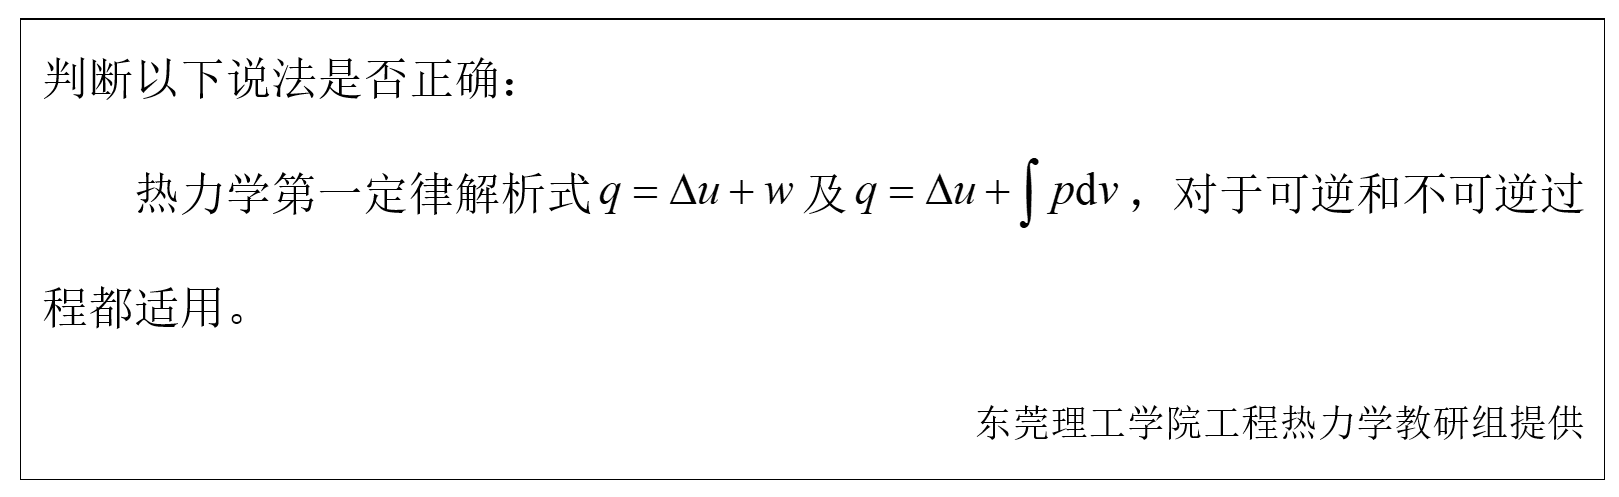
\includegraphics[width=0.8\textwidth, height=0.25\textheight, keepaspectratio]{question_1_17718566/title_img_1.png}\end{center}

\textbf{正确答案:}
false

\vspace{0.5em}\hrulefill\vspace{1em}

\subsection*{2. (填空题/简答题) \small ID: 17718570}

\textbf{题干:}


\begin{center}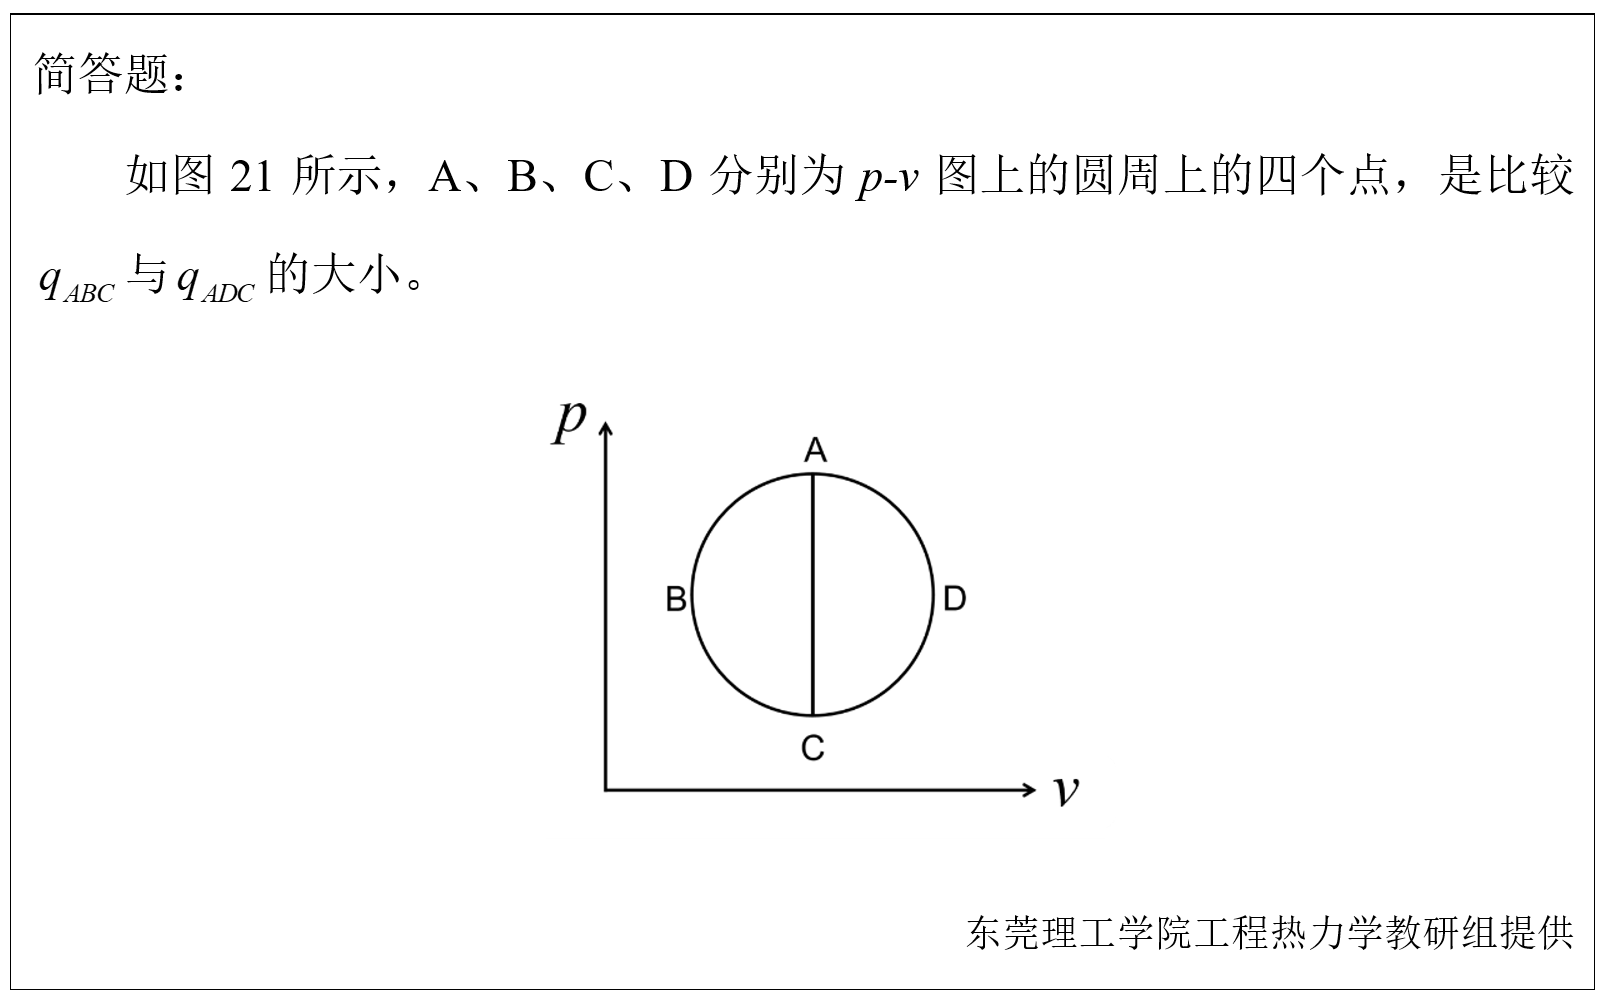
\includegraphics[width=0.8\textwidth, height=0.25\textheight, keepaspectratio]{question_2_17718570/title_img_1.png}\end{center}

\textbf{正确答案:}

\begin{center}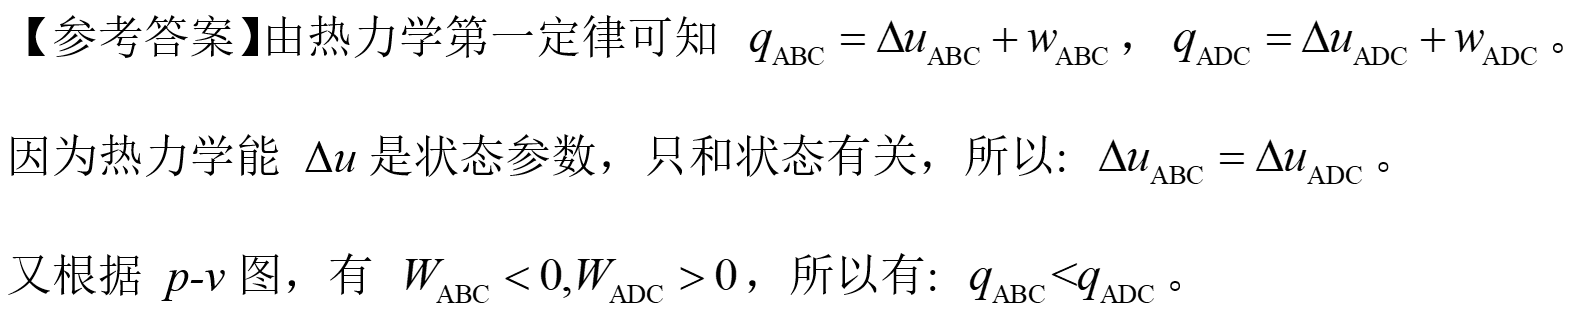
\includegraphics[width=0.7\textwidth, height=0.2\textheight, keepaspectratio]{question_2_17718570/correct_answer_1_img_1.png}\end{center}

\vspace{0.5em}\hrulefill\vspace{1em}

\subsection*{3. (判断题) \small ID: 17718564}

\textbf{题干:}


\begin{center}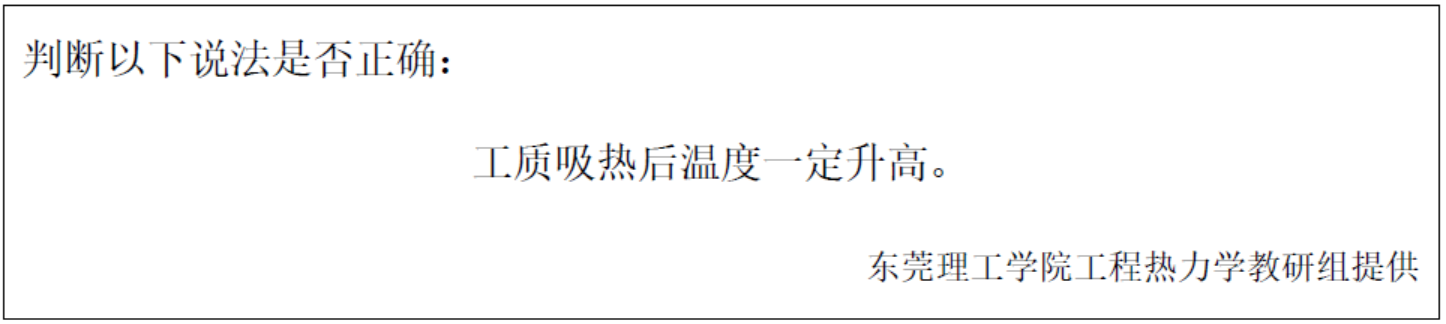
\includegraphics[width=0.8\textwidth, height=0.25\textheight, keepaspectratio]{question_3_17718564/title_img_1.png}\end{center}

\textbf{正确答案:}
false

\vspace{0.5em}\hrulefill\vspace{1em}

\subsection*{4. (判断题) \small ID: 17718562}

\textbf{题干:}


\begin{center}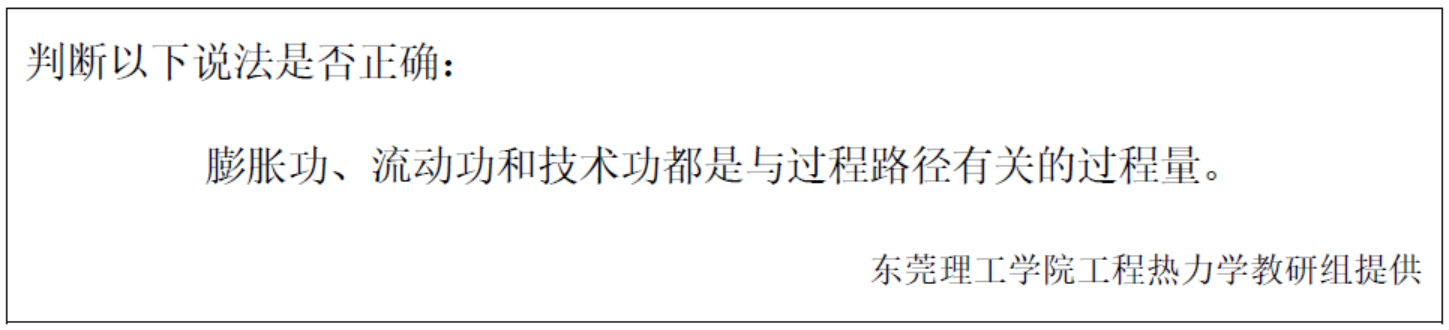
\includegraphics[width=0.8\textwidth, height=0.25\textheight, keepaspectratio]{question_4_17718562/title_img_1.png}\end{center}

\textbf{正确答案:}
false

\vspace{0.5em}\hrulefill\vspace{1em}

\subsection*{5. (判断题) \small ID: 17718565}

\textbf{题干:}


\begin{center}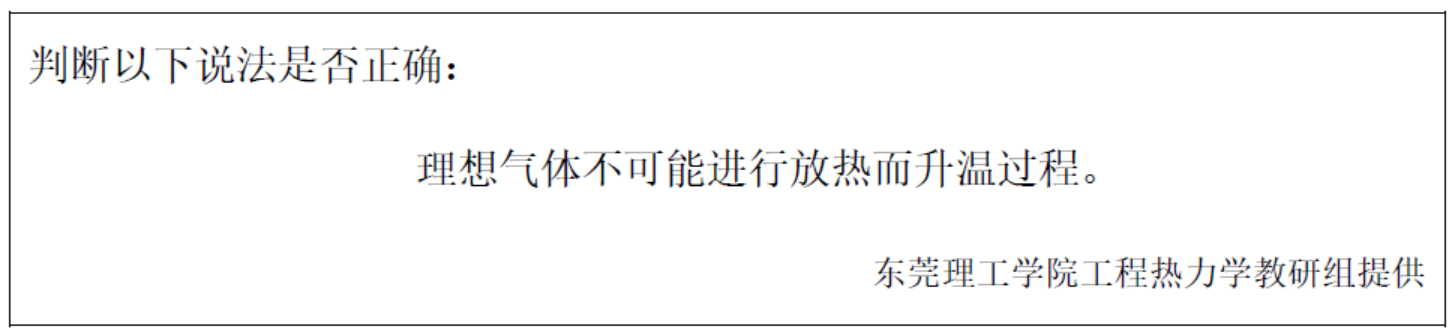
\includegraphics[width=0.8\textwidth, height=0.25\textheight, keepaspectratio]{question_5_17718565/title_img_1.png}\end{center}

\textbf{正确答案:}
false

\vspace{0.5em}\hrulefill\vspace{1em}

\subsection*{6. (单选题) \small ID: 17718552}

\textbf{题干:}


\begin{center}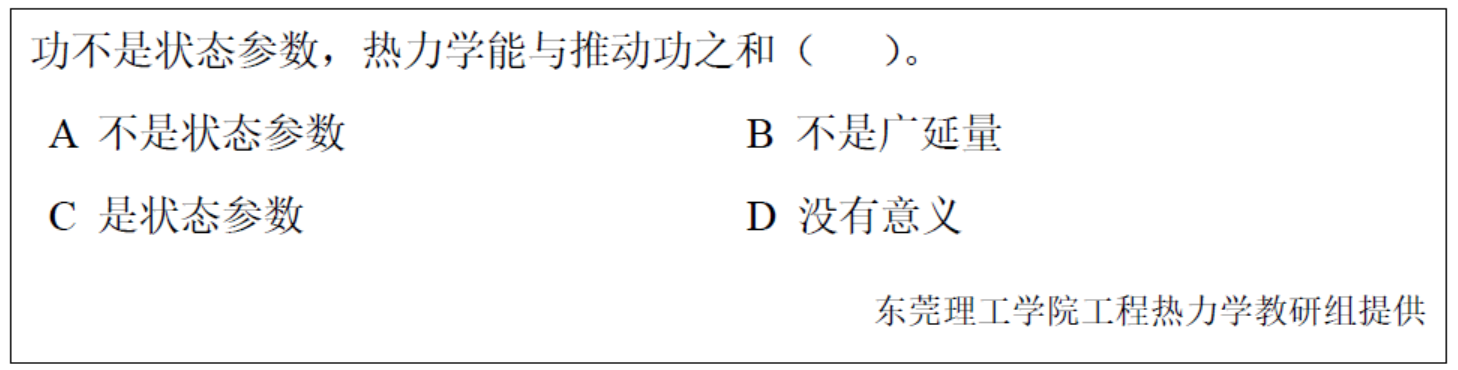
\includegraphics[width=0.8\textwidth, height=0.25\textheight, keepaspectratio]{question_6_17718552/title_img_1.png}\end{center}

\textbf{选项:}
\begin{itemize}[leftmargin=*]
  \item A

  \item B

  \item C

  \item D

\end{itemize}

\textbf{正确答案:}
C

\vspace{0.5em}\hrulefill\vspace{1em}

\subsection*{7. (填空题/简答题) \small ID: 17718575}

\textbf{题干:}


\begin{center}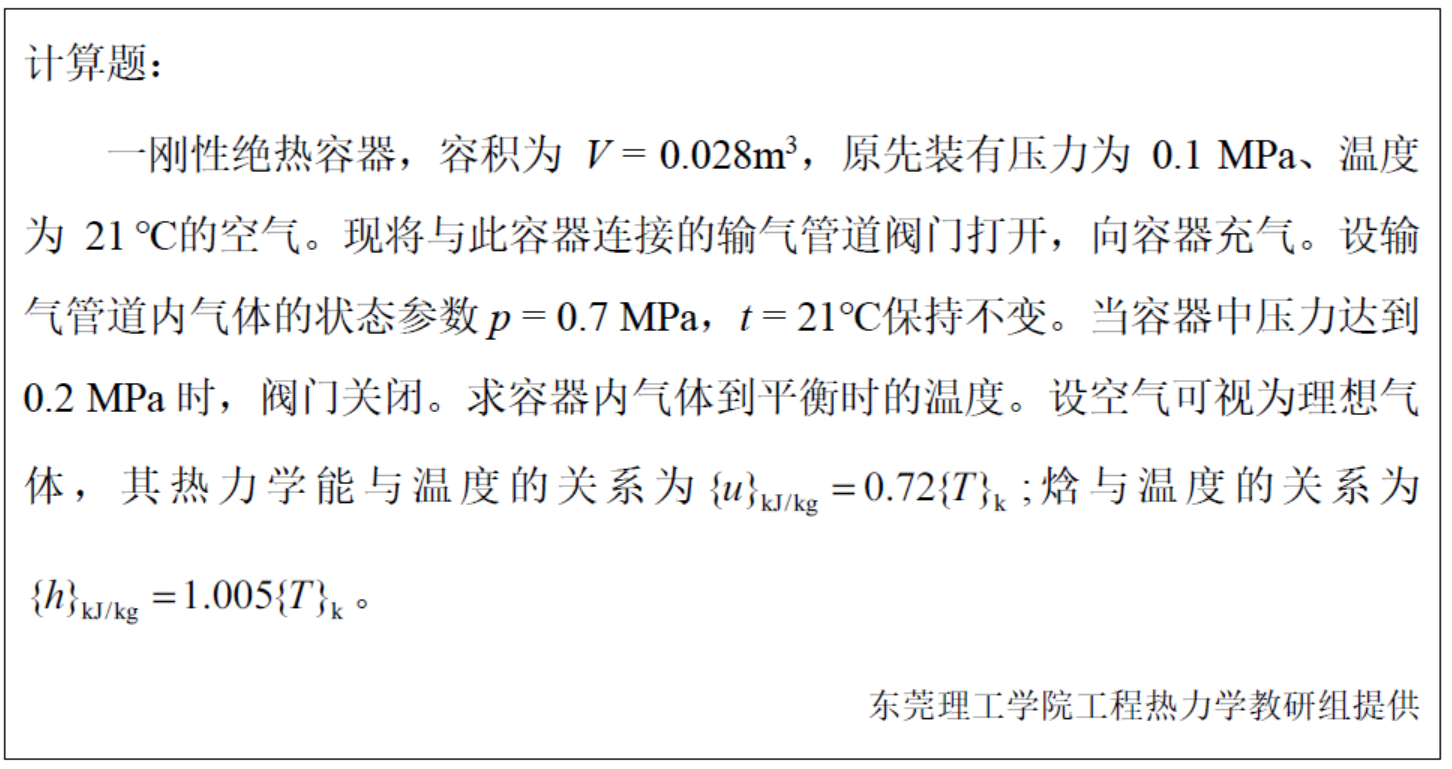
\includegraphics[width=0.8\textwidth, height=0.25\textheight, keepaspectratio]{question_7_17718575/title_img_1.png}\end{center}

\textbf{正确答案:}

\begin{center}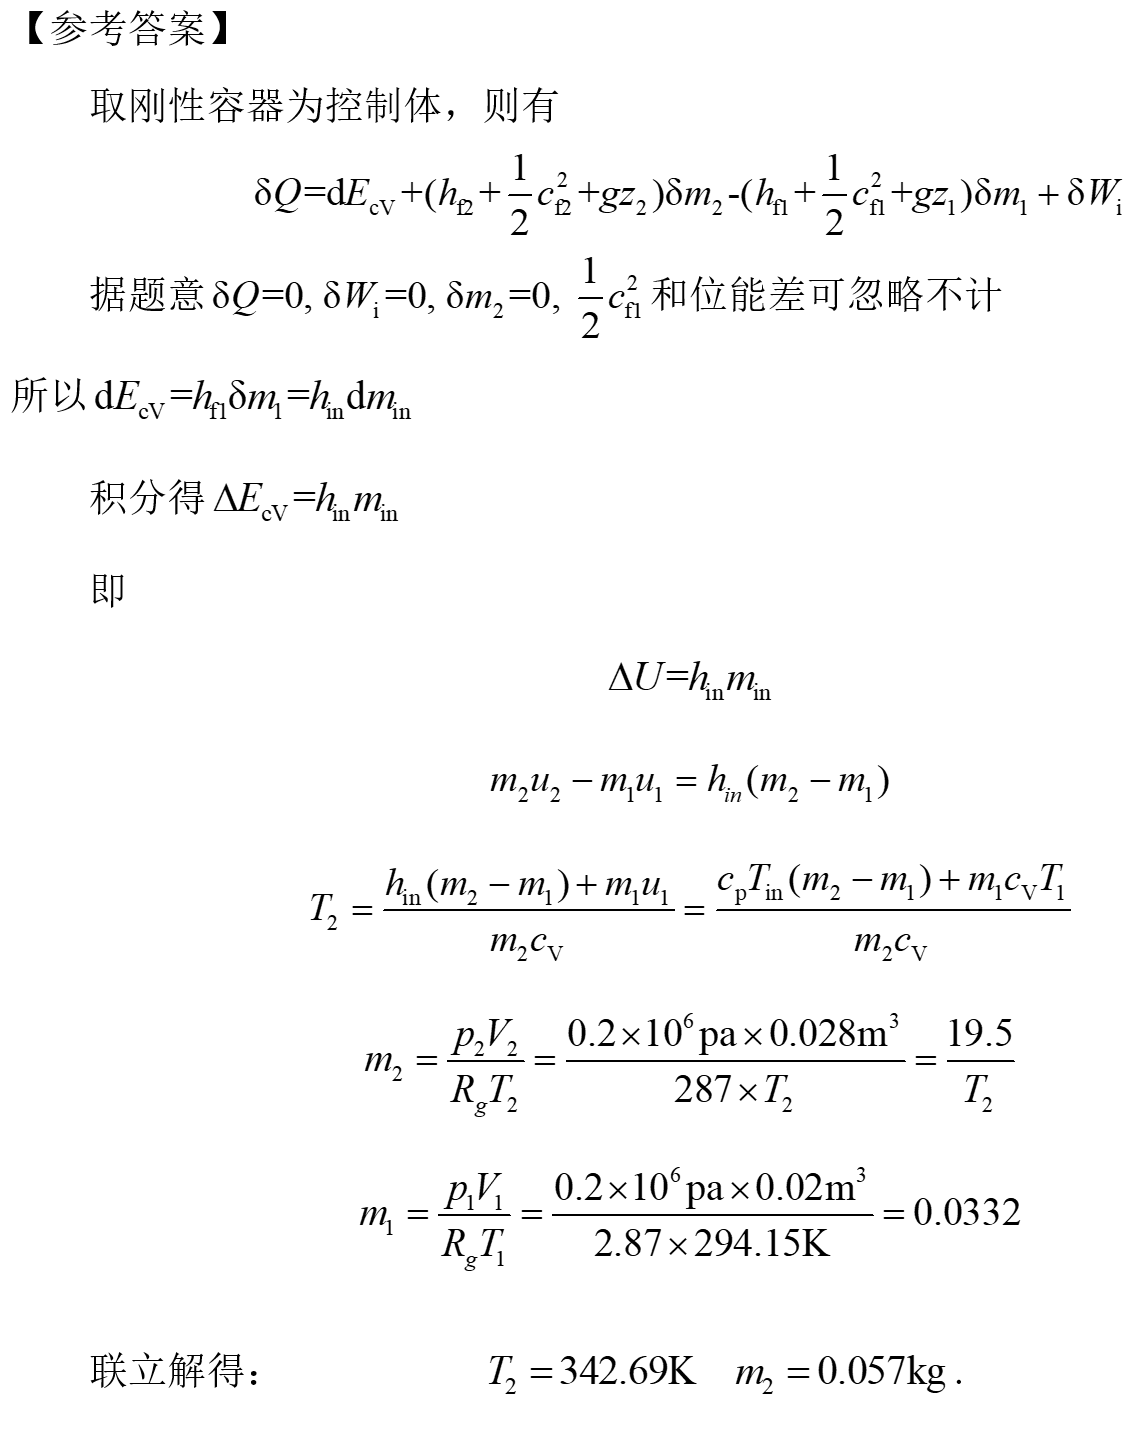
\includegraphics[width=0.7\textwidth, height=0.2\textheight, keepaspectratio]{question_7_17718575/correct_answer_1_img_1.png}\end{center}

\vspace{0.5em}\hrulefill\vspace{1em}

\subsection*{8. (判断题) \small ID: 17718560}

\textbf{题干:}


\begin{center}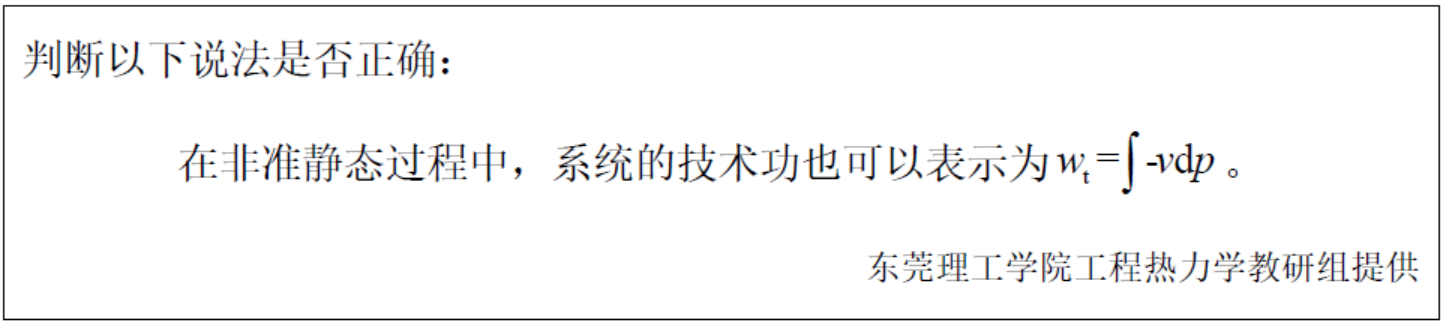
\includegraphics[width=0.8\textwidth, height=0.25\textheight, keepaspectratio]{question_8_17718560/title_img_1.png}\end{center}

\textbf{正确答案:}
false

\vspace{0.5em}\hrulefill\vspace{1em}

\subsection*{9. (不定项选择题) \small ID: 17718569}

\textbf{题干:}

答案为:( ),( )
\begin{center}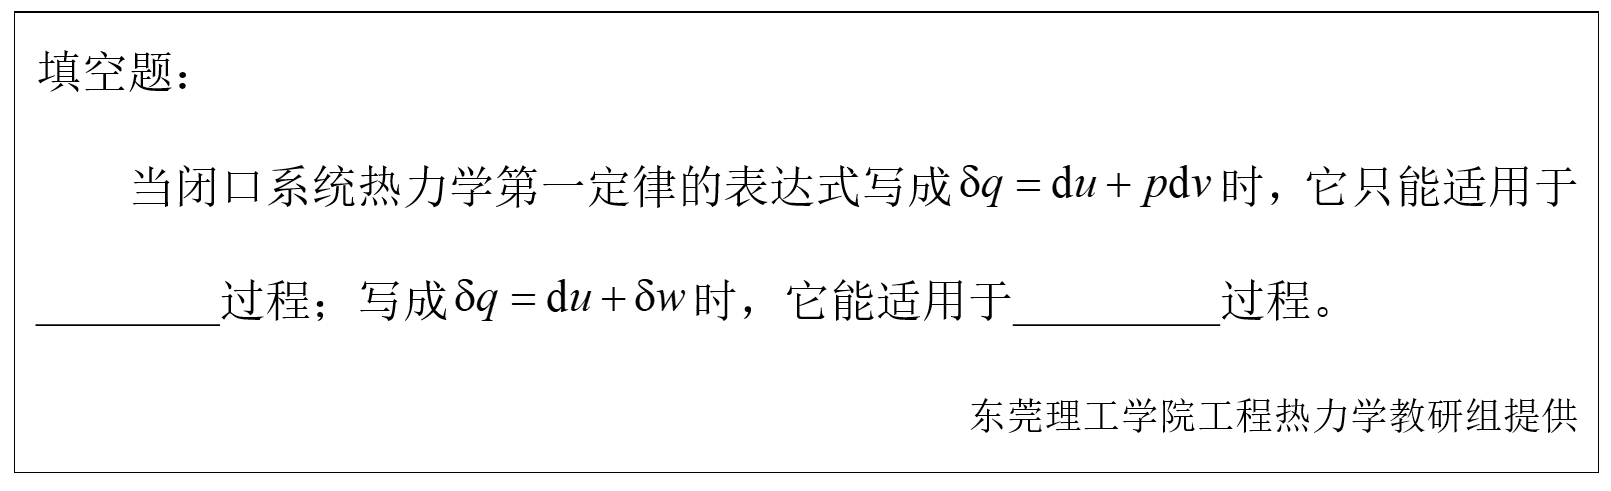
\includegraphics[width=0.8\textwidth, height=0.25\textheight, keepaspectratio]{question_9_17718569/title_img_1.png}\end{center}

\textbf{正确答案:}
准静态
任何

\vspace{0.5em}\hrulefill\vspace{1em}

\subsection*{10. (判断题) \small ID: 17718568}

\textbf{题干:}


\begin{center}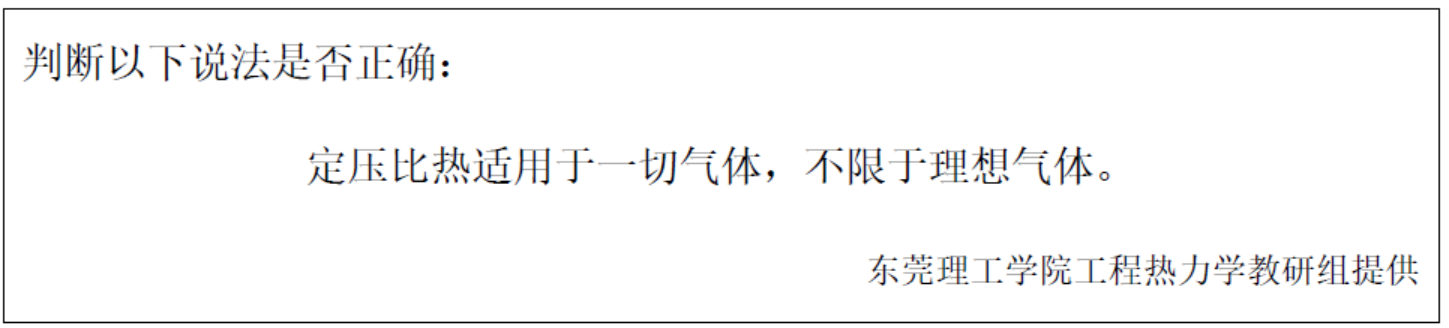
\includegraphics[width=0.8\textwidth, height=0.25\textheight, keepaspectratio]{question_10_17718568/title_img_1.png}\end{center}

\textbf{正确答案:}
true

\vspace{0.5em}\hrulefill\vspace{1em}

\subsection*{11. (判断题) \small ID: 17718558}

\textbf{题干:}


\begin{center}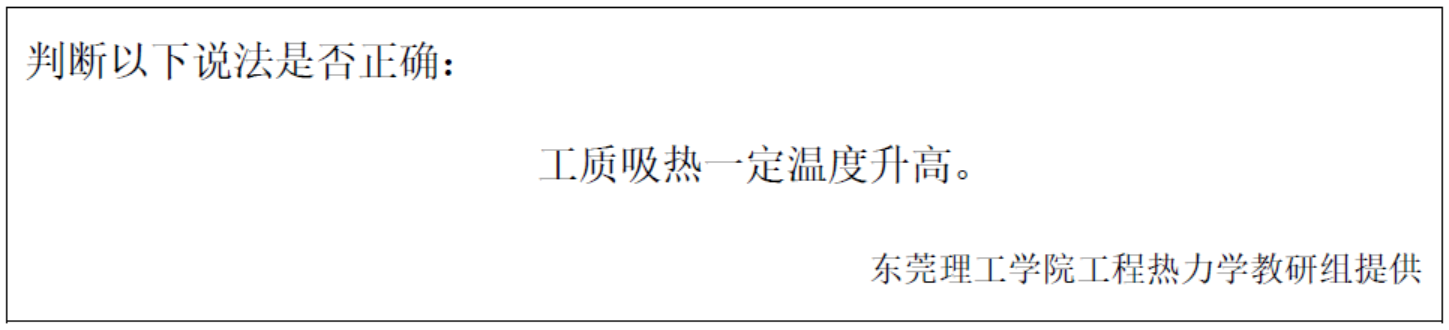
\includegraphics[width=0.8\textwidth, height=0.25\textheight, keepaspectratio]{question_11_17718558/title_img_1.png}\end{center}

\textbf{正确答案:}
false

\vspace{0.5em}\hrulefill\vspace{1em}

\subsection*{12. (填空题/简答题) \small ID: 17718576}

\textbf{题干:}


\begin{center}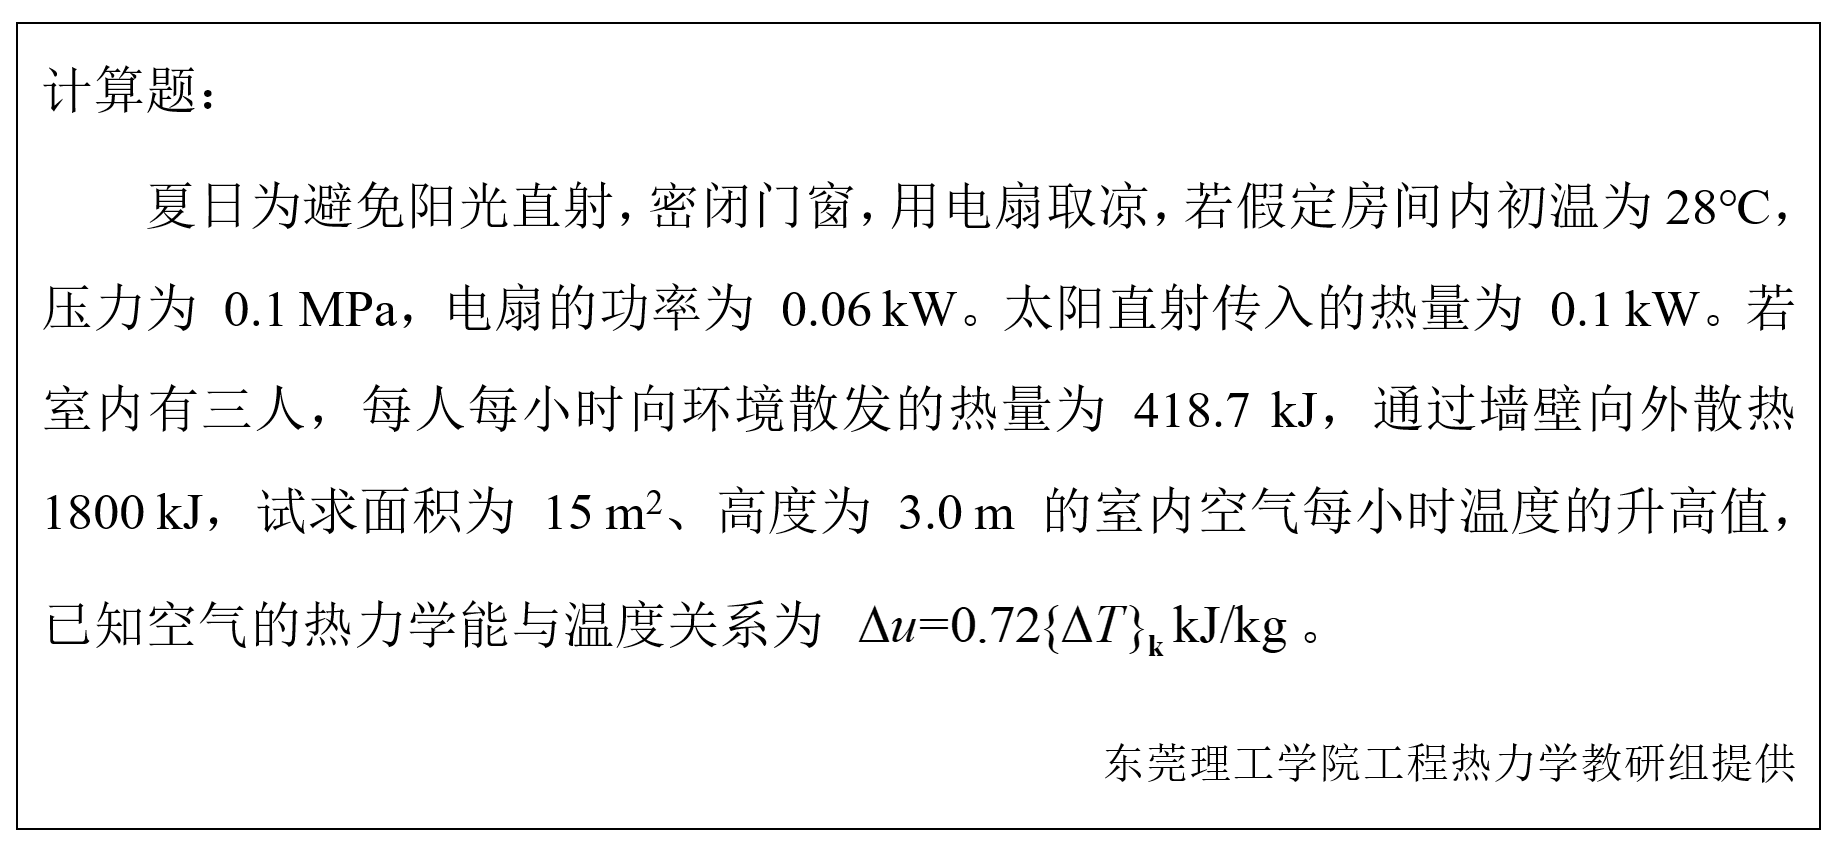
\includegraphics[width=0.8\textwidth, height=0.25\textheight, keepaspectratio]{question_12_17718576/title_img_1.png}\end{center}

\textbf{正确答案:}

\begin{center}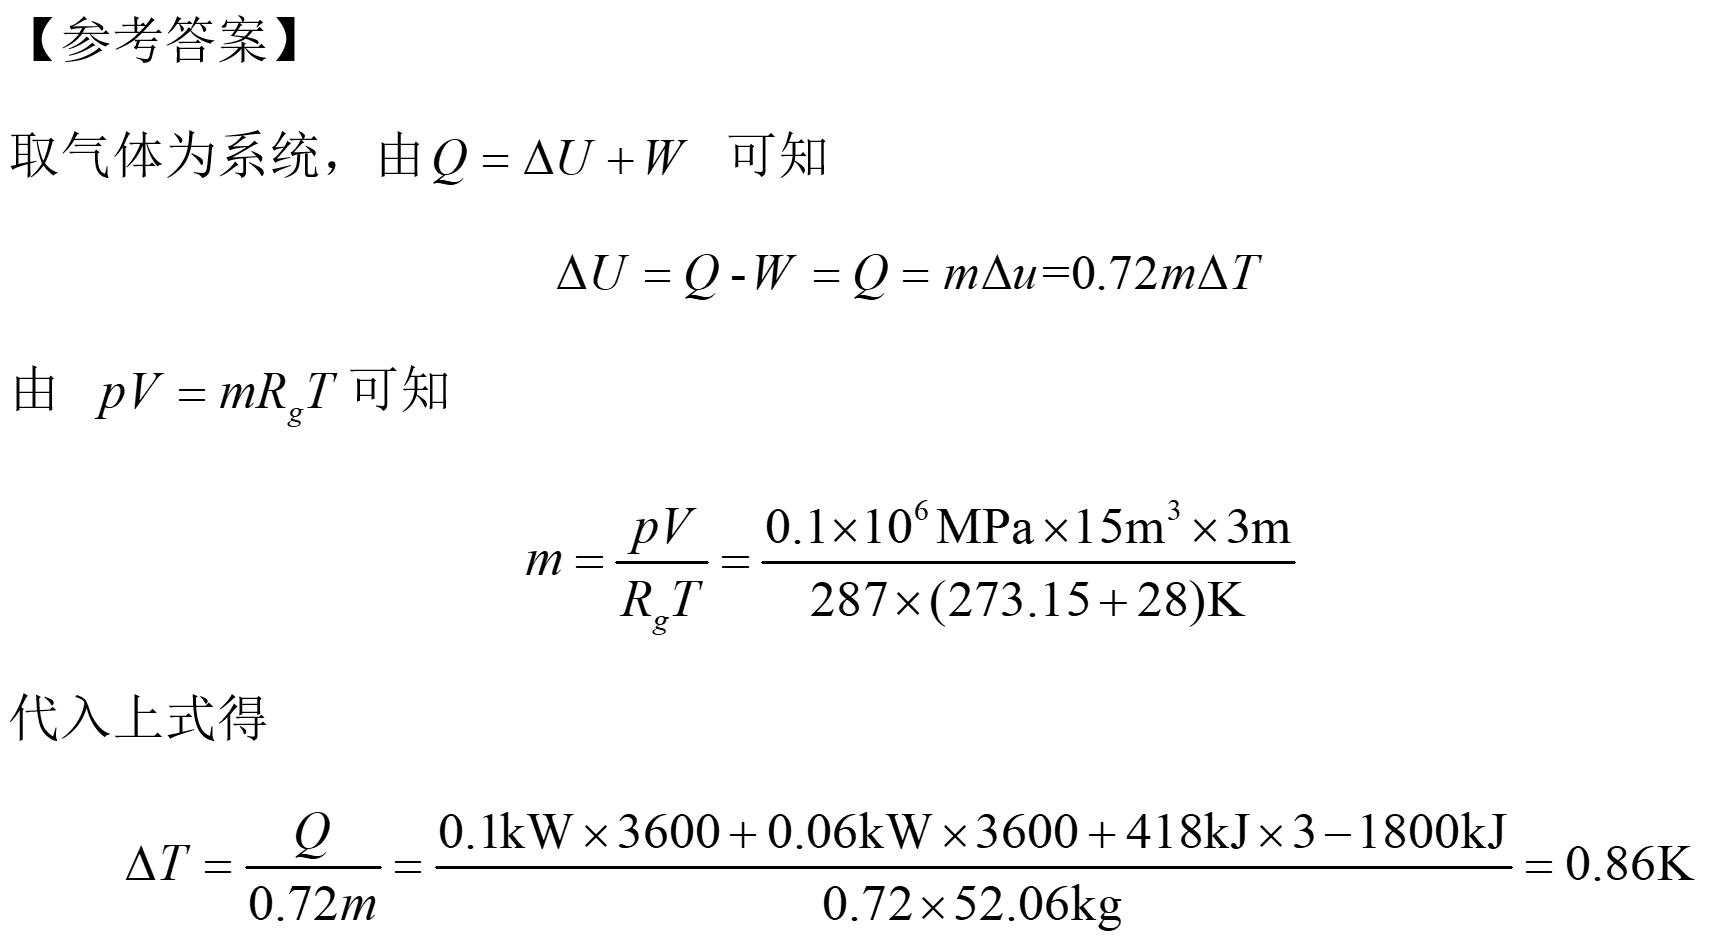
\includegraphics[width=0.7\textwidth, height=0.2\textheight, keepaspectratio]{question_12_17718576/correct_answer_1_img_1.png}\end{center}

\vspace{0.5em}\hrulefill\vspace{1em}

\subsection*{13. (判断题) \small ID: 17718567}

\textbf{题干:}


\begin{center}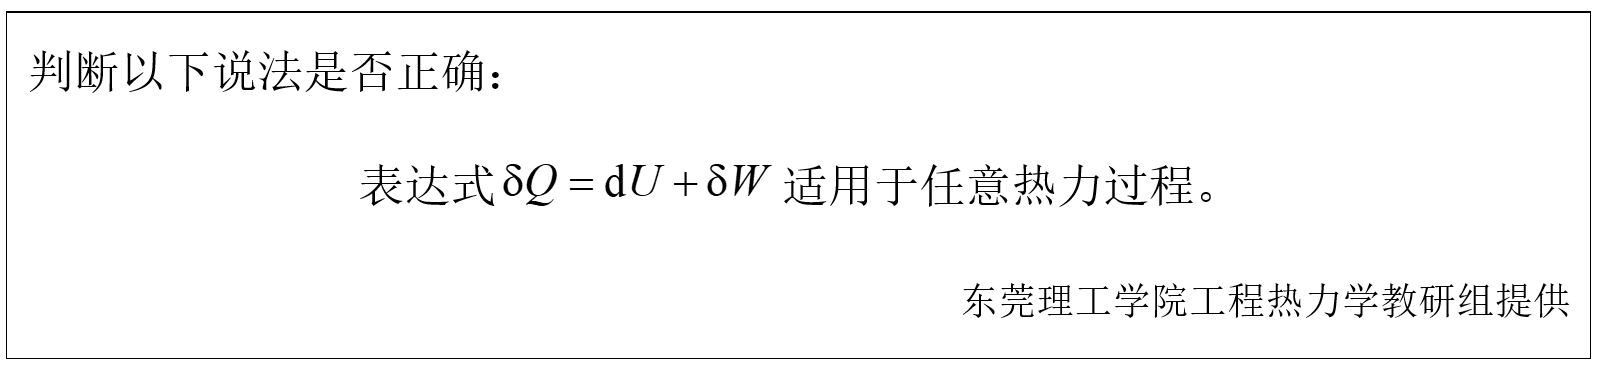
\includegraphics[width=0.8\textwidth, height=0.25\textheight, keepaspectratio]{question_13_17718567/title_img_1.png}\end{center}

\textbf{正确答案:}
true

\vspace{0.5em}\hrulefill\vspace{1em}

\subsection*{14. (单选题) \small ID: 17718557}

\textbf{题干:}


\begin{center}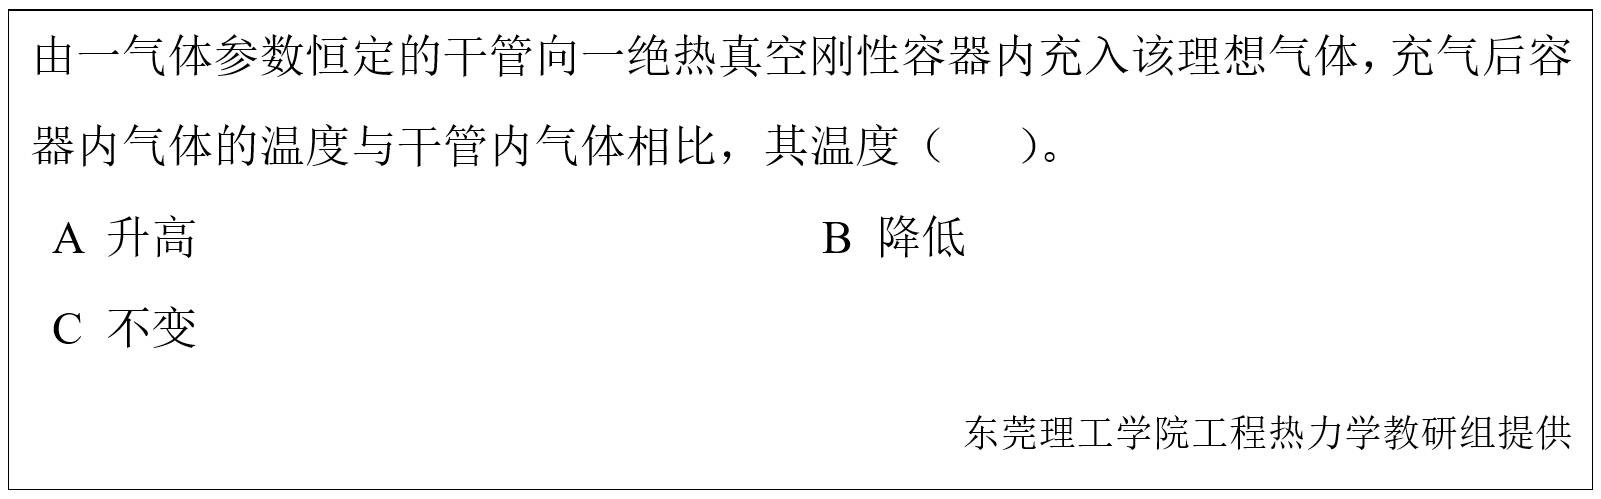
\includegraphics[width=0.8\textwidth, height=0.25\textheight, keepaspectratio]{question_14_17718557/title_img_1.png}\end{center}

\textbf{选项:}
\begin{itemize}[leftmargin=*]
  \item A

  \item B

  \item C

\end{itemize}

\textbf{正确答案:}
A

\textbf{答案解析:}

充气的过程中增加了流动功,故导致瓶子气体的内能升高,温度升高。

\vspace{0.5em}\hrulefill\vspace{1em}

\subsection*{15. (判断题) \small ID: 17718563}

\textbf{题干:}


\begin{center}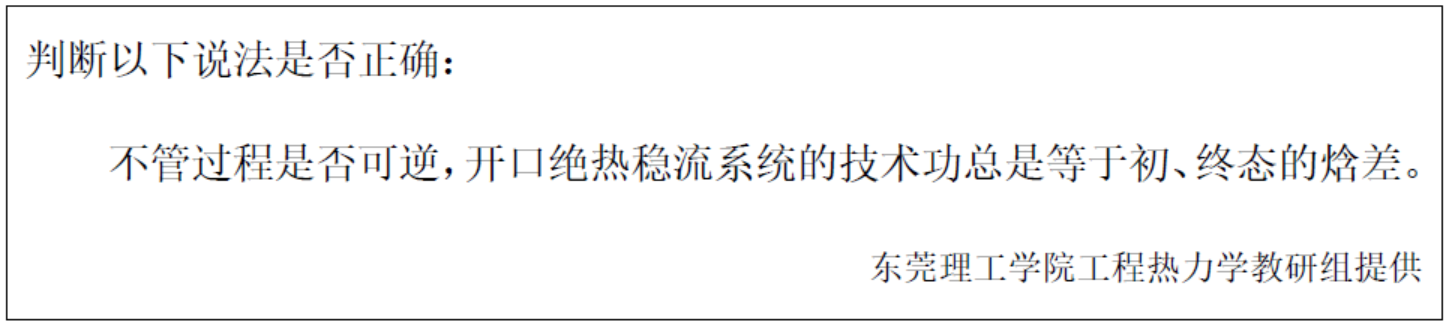
\includegraphics[width=0.8\textwidth, height=0.25\textheight, keepaspectratio]{question_15_17718563/title_img_1.png}\end{center}

\textbf{正确答案:}
true

\vspace{0.5em}\hrulefill\vspace{1em}

\subsection*{16. (单选题) \small ID: 17718549}

\textbf{题干:}


\begin{center}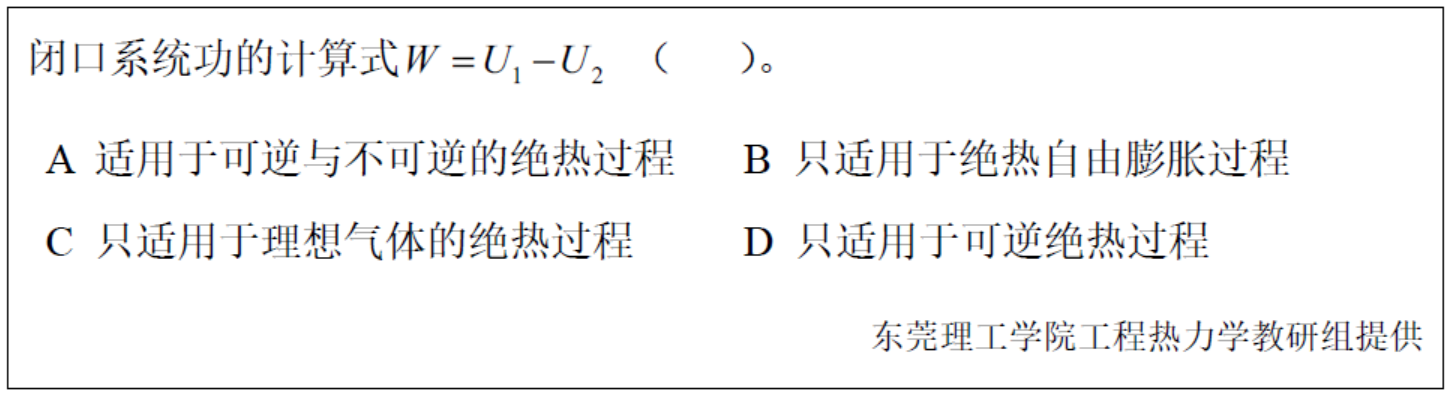
\includegraphics[width=0.8\textwidth, height=0.25\textheight, keepaspectratio]{question_16_17718549/title_img_1.png}\end{center}

\textbf{选项:}
\begin{itemize}[leftmargin=*]
  \item A

  \item B

  \item C

  \item D

\end{itemize}

\textbf{正确答案:}
A

\vspace{0.5em}\hrulefill\vspace{1em}

\subsection*{17. (填空题/简答题) \small ID: 17718574}

\textbf{题干:}


\begin{center}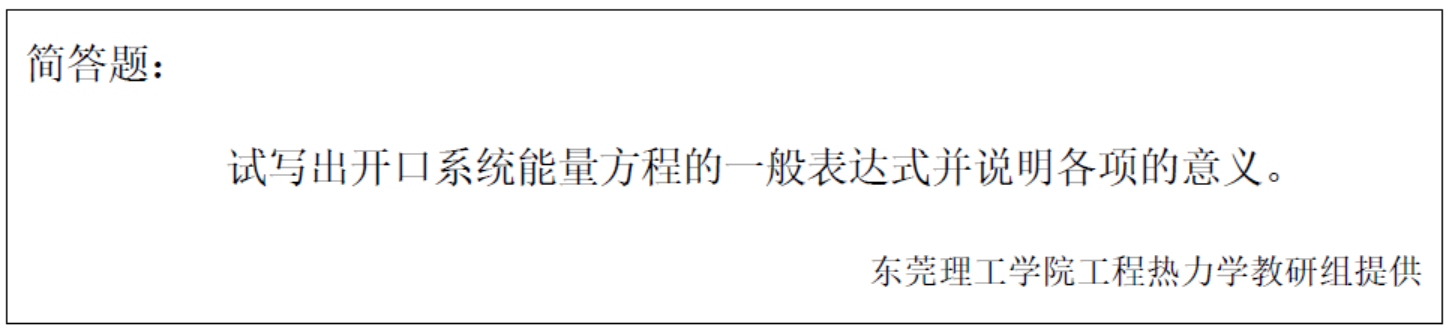
\includegraphics[width=0.8\textwidth, height=0.25\textheight, keepaspectratio]{question_17_17718574/title_img_1.png}\end{center}

\textbf{正确答案:}

\begin{center}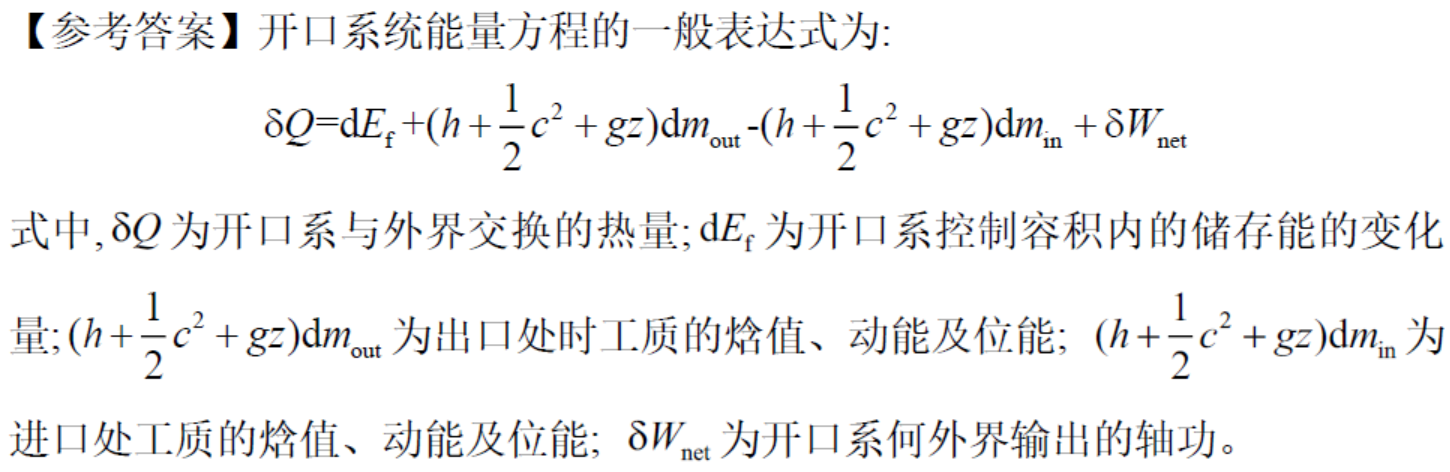
\includegraphics[width=0.7\textwidth, height=0.2\textheight, keepaspectratio]{question_17_17718574/correct_answer_1_img_1.png}\end{center}

\vspace{0.5em}\hrulefill\vspace{1em}

\subsection*{18. (单选题) \small ID: 17718554}

\textbf{题干:}


\begin{center}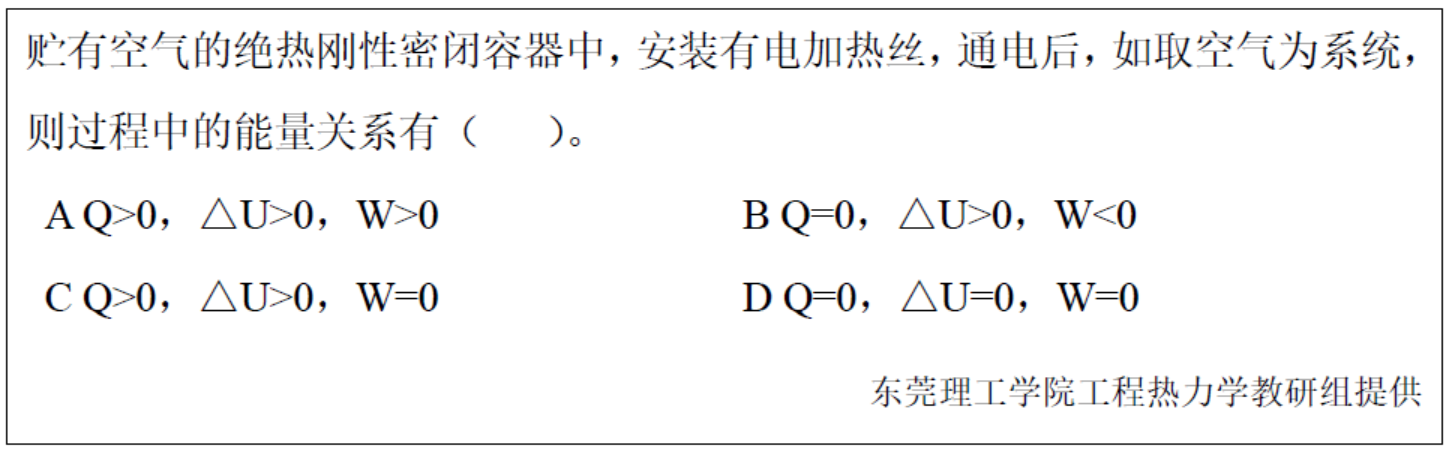
\includegraphics[width=0.8\textwidth, height=0.25\textheight, keepaspectratio]{question_18_17718554/title_img_1.png}\end{center}

\textbf{选项:}
\begin{itemize}[leftmargin=*]
  \item A

  \item B

  \item C

  \item D

\end{itemize}

\textbf{正确答案:}
C

\vspace{0.5em}\hrulefill\vspace{1em}

\subsection*{19. (单选题) \small ID: 17718556}

\textbf{题干:}


\begin{center}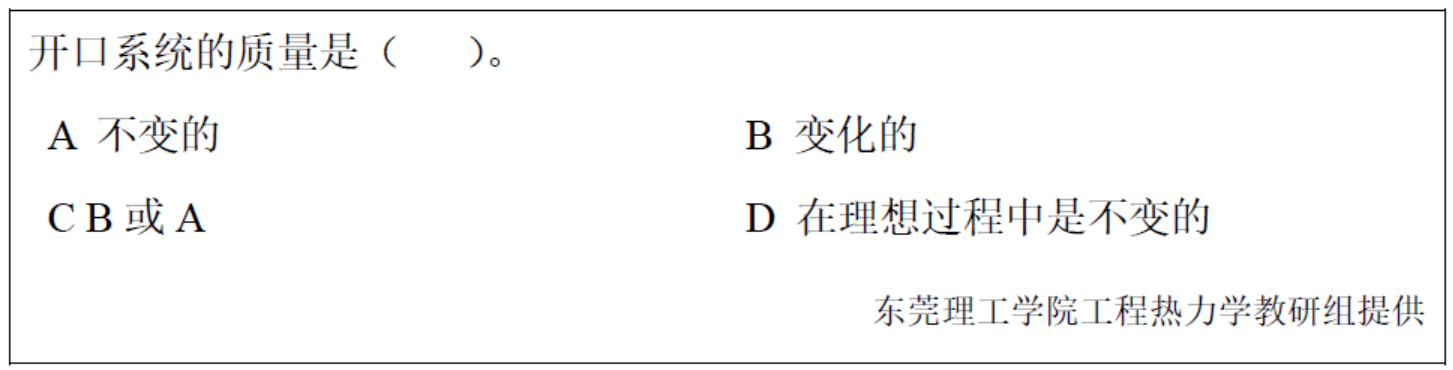
\includegraphics[width=0.8\textwidth, height=0.25\textheight, keepaspectratio]{question_19_17718556/title_img_1.png}\end{center}

\textbf{选项:}
\begin{itemize}[leftmargin=*]
  \item A

  \item B

  \item C

  \item D

\end{itemize}

\textbf{正确答案:}
C

\vspace{0.5em}\hrulefill\vspace{1em}

\subsection*{20. (单选题) \small ID: 17718555}

\textbf{题干:}


\begin{center}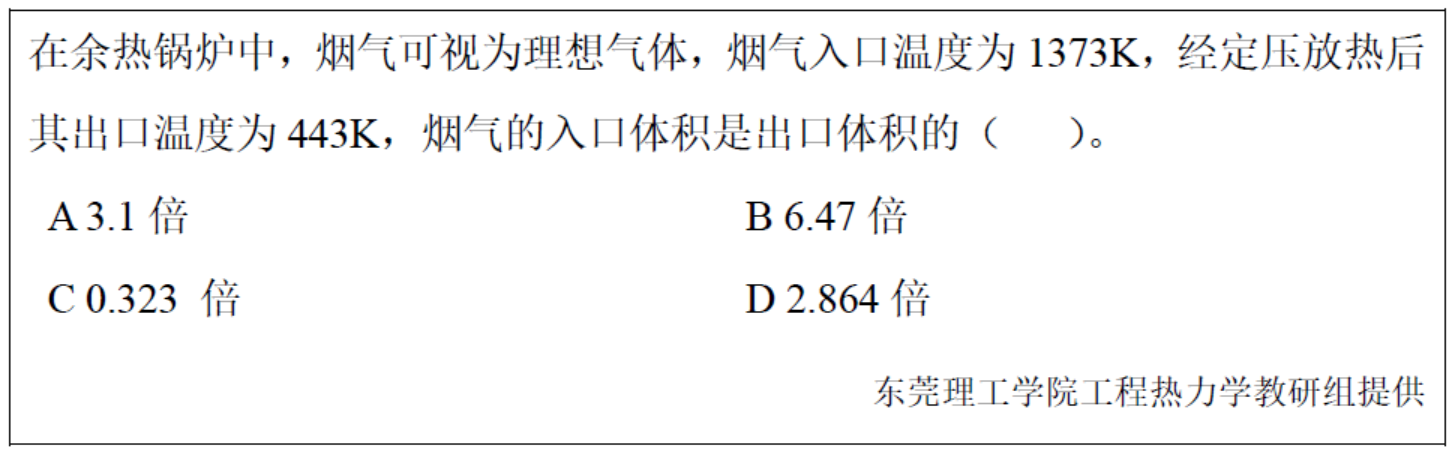
\includegraphics[width=0.8\textwidth, height=0.25\textheight, keepaspectratio]{question_20_17718555/title_img_1.png}\end{center}

\textbf{选项:}
\begin{itemize}[leftmargin=*]
  \item A

  \item B

  \item C

  \item D

\end{itemize}

\textbf{正确答案:}
A

\vspace{0.5em}\hrulefill\vspace{1em}

\subsection*{21. (单选题) \small ID: 17718553}

\textbf{题干:}


\begin{center}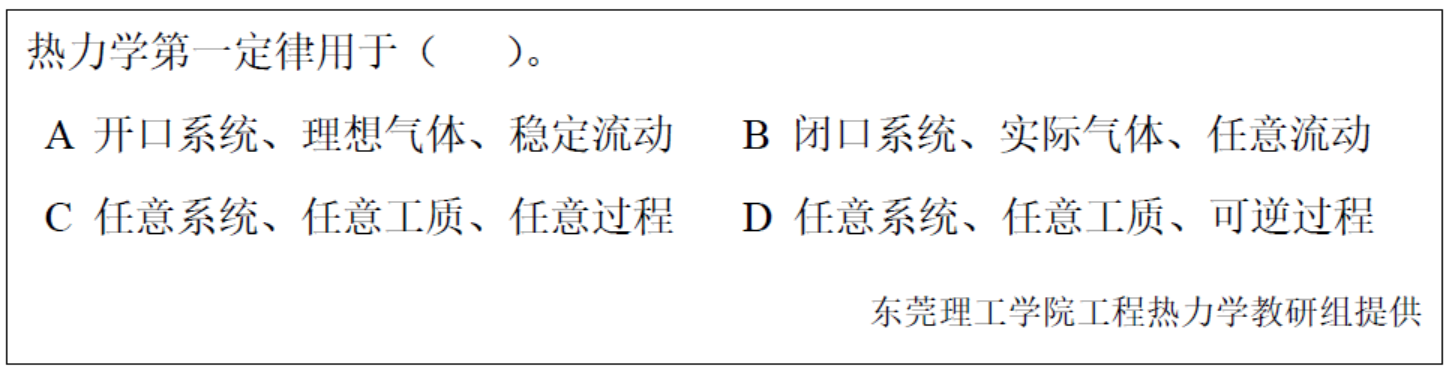
\includegraphics[width=0.8\textwidth, height=0.25\textheight, keepaspectratio]{question_21_17718553/title_img_1.png}\end{center}

\textbf{选项:}
\begin{itemize}[leftmargin=*]
  \item A

  \item B

  \item C

  \item D

\end{itemize}

\textbf{正确答案:}
C

\vspace{0.5em}\hrulefill\vspace{1em}

\subsection*{22. (判断题) \small ID: 17718561}

\textbf{题干:}


\begin{center}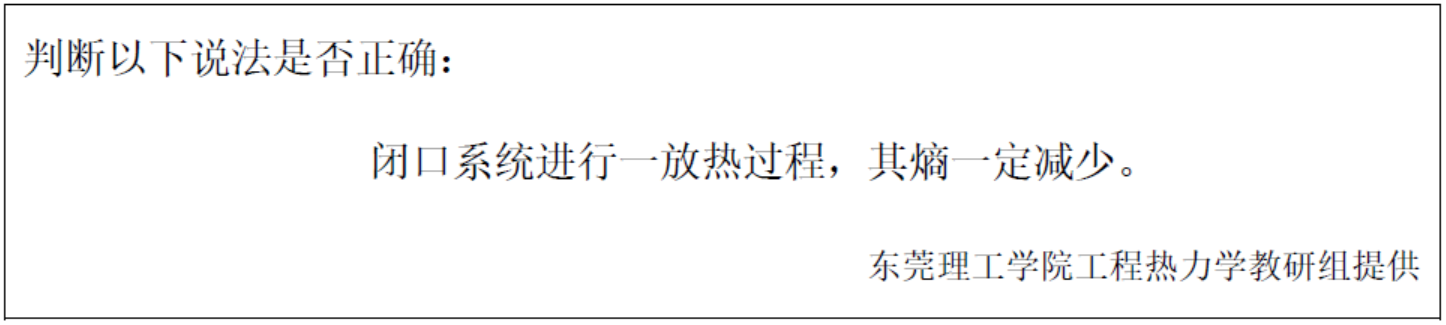
\includegraphics[width=0.8\textwidth, height=0.25\textheight, keepaspectratio]{question_22_17718561/title_img_1.png}\end{center}

\textbf{正确答案:}
false

\vspace{0.5em}\hrulefill\vspace{1em}

\subsection*{23. (判断题) \small ID: 17718559}

\textbf{题干:}


\begin{center}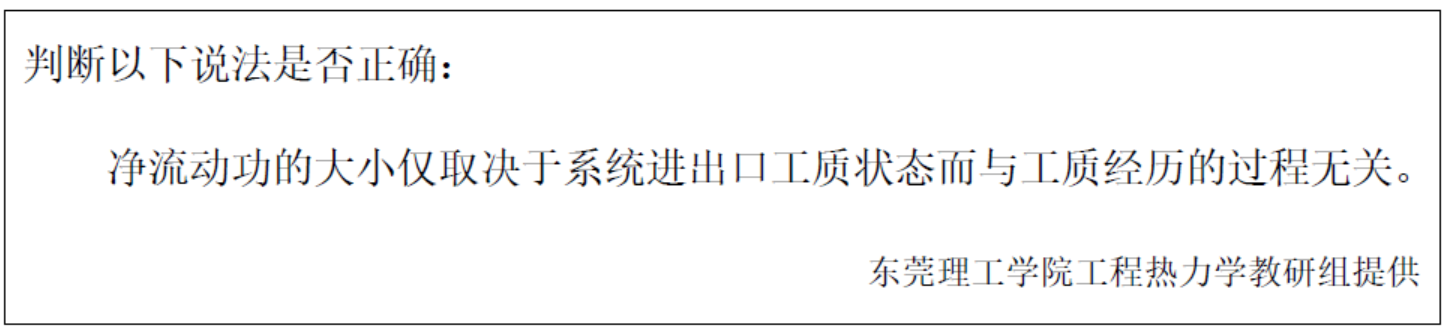
\includegraphics[width=0.8\textwidth, height=0.25\textheight, keepaspectratio]{question_23_17718559/title_img_1.png}\end{center}

\textbf{正确答案:}
true

\vspace{0.5em}\hrulefill\vspace{1em}

\subsection*{24. (单选题) \small ID: 17718550}

\textbf{题干:}


\begin{center}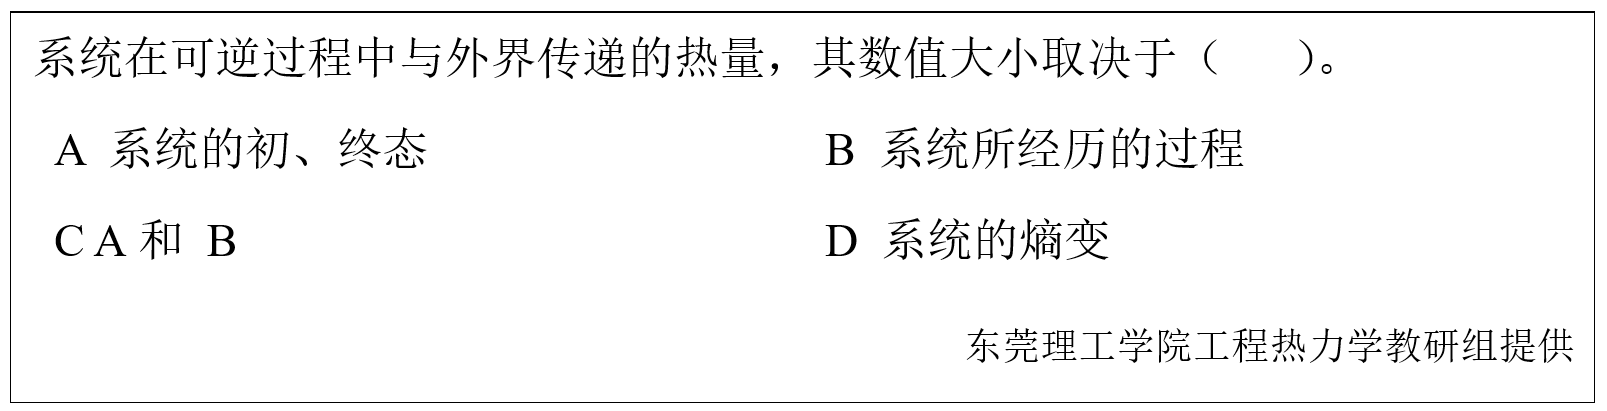
\includegraphics[width=0.8\textwidth, height=0.25\textheight, keepaspectratio]{question_24_17718550/title_img_1.png}\end{center}

\textbf{选项:}
\begin{itemize}[leftmargin=*]
  \item A

  \item B

  \item C

  \item D

\end{itemize}

\textbf{正确答案:}
C

\vspace{0.5em}\hrulefill\vspace{1em}

\subsection*{25. (填空题/简答题) \small ID: 17718572}

\textbf{题干:}


\begin{center}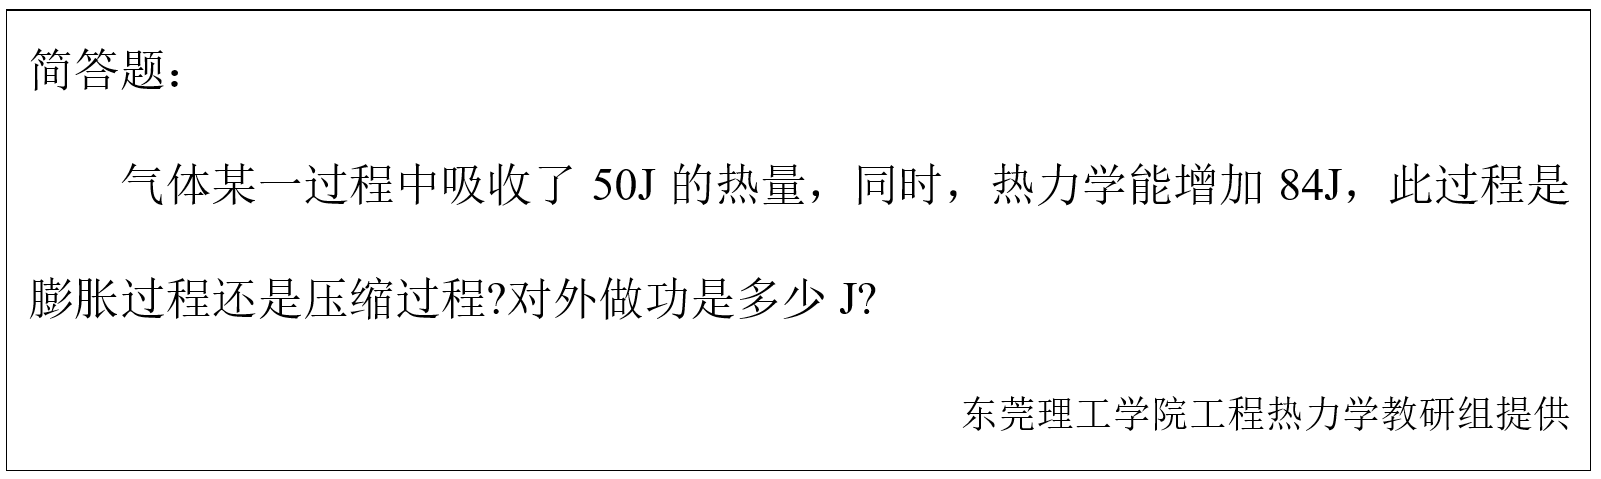
\includegraphics[width=0.8\textwidth, height=0.25\textheight, keepaspectratio]{question_25_17718572/title_img_1.png}\end{center}

\textbf{正确答案:}

\begin{center}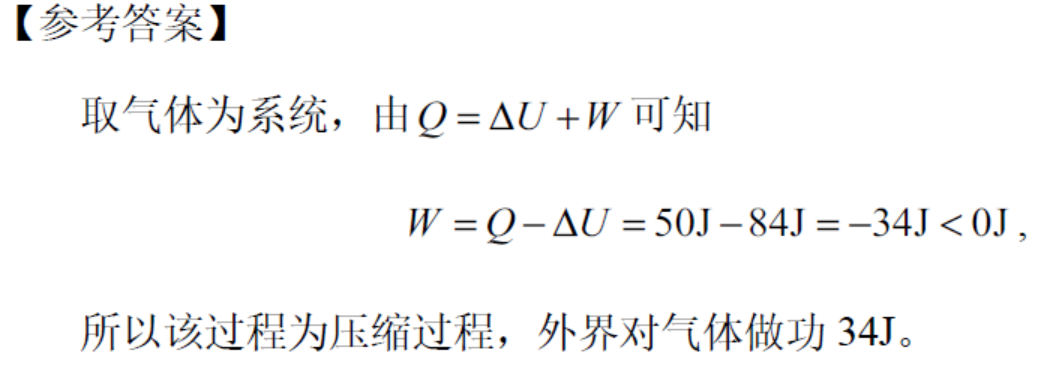
\includegraphics[width=0.7\textwidth, height=0.2\textheight, keepaspectratio]{question_25_17718572/correct_answer_1_img_1.png}\end{center}

\vspace{0.5em}\hrulefill\vspace{1em}

\subsection*{26. (填空题/简答题) \small ID: 17718573}

\textbf{题干:}


\begin{center}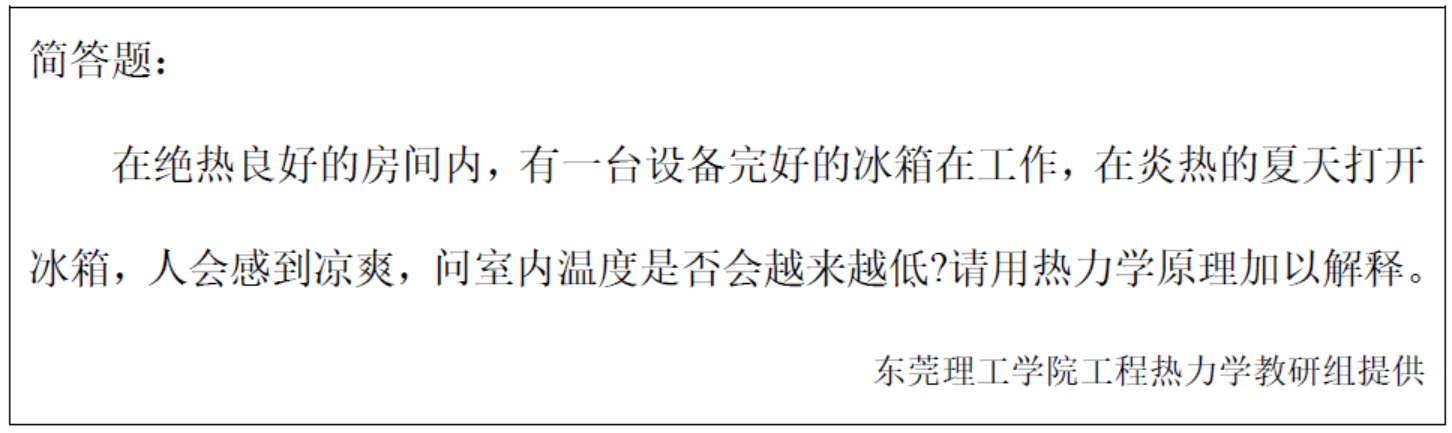
\includegraphics[width=0.8\textwidth, height=0.25\textheight, keepaspectratio]{question_26_17718573/title_img_1.png}\end{center}

\textbf{正确答案:}

\begin{center}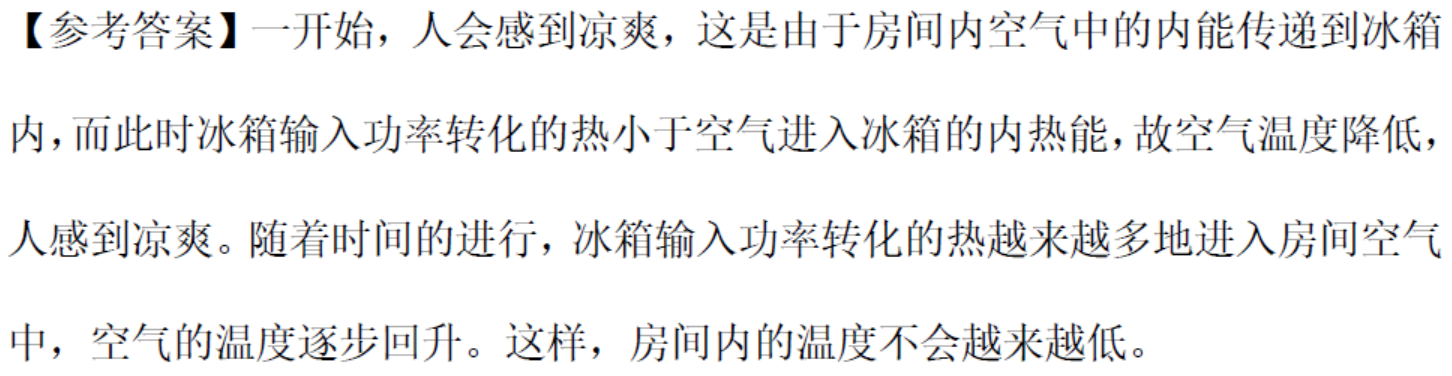
\includegraphics[width=0.7\textwidth, height=0.2\textheight, keepaspectratio]{question_26_17718573/correct_answer_1_img_1.png}\end{center}

\vspace{0.5em}\hrulefill\vspace{1em}

\subsection*{27. (单选题) \small ID: 17718551}

\textbf{题干:}


\begin{center}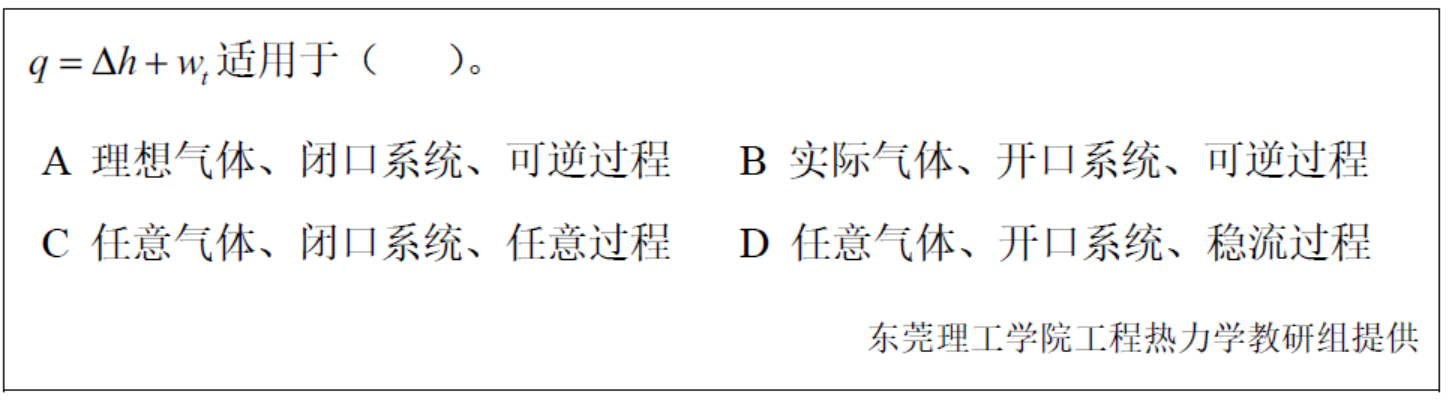
\includegraphics[width=0.8\textwidth, height=0.25\textheight, keepaspectratio]{question_27_17718551/title_img_1.png}\end{center}

\textbf{选项:}
\begin{itemize}[leftmargin=*]
  \item A

  \item B

  \item C

  \item D

\end{itemize}

\textbf{正确答案:}
D

\vspace{0.5em}\hrulefill\vspace{1em}

\subsection*{28. (填空题/简答题) \small ID: 17718571}

\textbf{题干:}


\begin{center}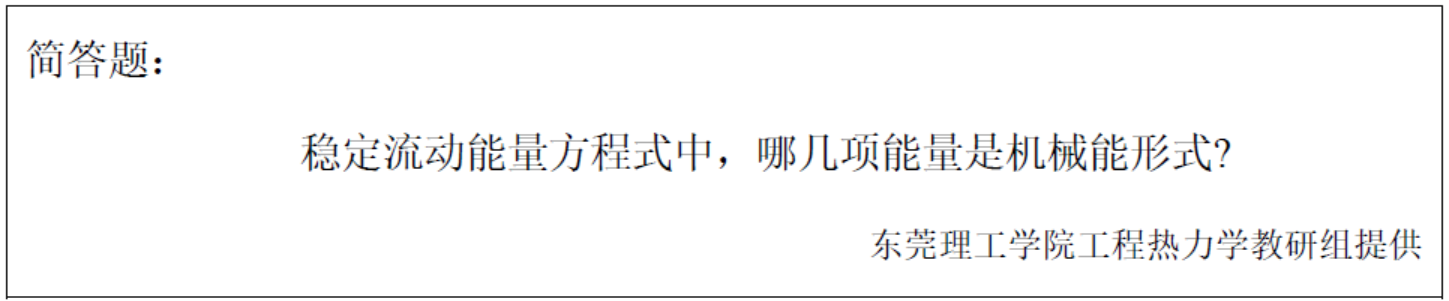
\includegraphics[width=0.8\textwidth, height=0.25\textheight, keepaspectratio]{question_28_17718571/title_img_1.png}\end{center}

\textbf{正确答案:}

\begin{center}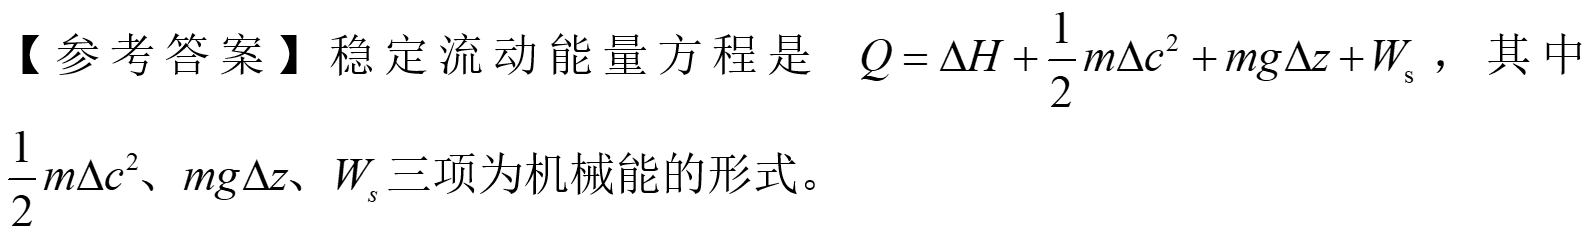
\includegraphics[width=0.7\textwidth, height=0.2\textheight, keepaspectratio]{question_28_17718571/correct_answer_1_img_1.png}\end{center}

\vspace{0.5em}\hrulefill\vspace{1em}

\end{document}
